% !TEX root = ../../Noctua_Diplomarbeit.tex

\subsection{Unterst�tzung und Widerstand}

Die Kurse von Aktien unterliegen, wie bereits erw�hnt, gewissen Trends, die entweder auf-, ab- oder auch seitw�rts (weder auf- noch abw�rts) verlaufen. Bei steigenden Kursen erreichen diese irgendwann ein Level, bei dem der Preis nicht mehr als billig angesehen wird und der Kurs dreht sich um. Der Trend verliert also seine Nachhaltigkeit. Dieses Level wird als \emph{Widerstand} oder \emph{Resistance} bezeichnet, da es nur schwer �berwunden wird. Sinkt der Kurs eine Weile wieder und sonstige Bewertungskriterien des Handelsgutes haben sich nicht signifikant ver�ndert, erreicht der Kurs einen Punkt, bei dem er wieder interessant f�r etwaige K�ufer wird. Diese Schwelle wird als \emph{Unterst�tzung} oder \emph{Support} bezeichnet. \cite{elder_living} Am Beispiel von Microsoft kann diese Funktion in der Abbildung \ref{fig:msft_sup_res} �ber einen l�ngeren Zeitraum beobachtet werden\\

Diese beiden Schwellen sind tempor�re Hilfsmittel und lassen Wendepunkte erahnen. Beim Durchbruch eines Levels kann hingegen mit einer Fortsetzung dieses Trends gerechnet werden und ggf. wird ein alter Widerstand zur Unterst�tzung. \cite{investopedia-support-resistance} Abbildung \ref{fig:payx_sup_res} von Paychex Inc. veranschaulicht diesen Wechsel von Unterst�tzungs- zu Widerstands- und wieder zur�ck zu Unterst�tzungsleveln.

\begin{figure}
	\centering
		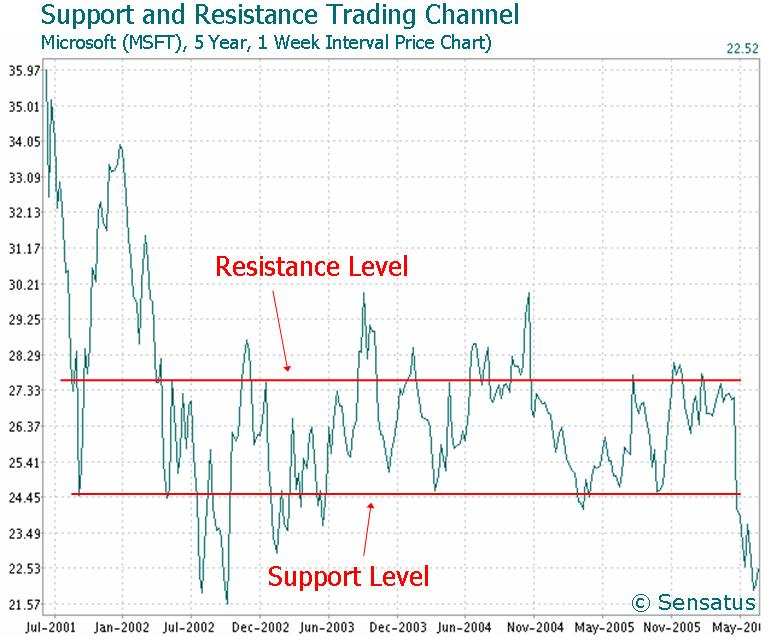
\includegraphics[width=0.8\textwidth]{graphics/fingrundlagen/msft_sup_res.JPG}
	\caption[Microsoft Support Resistance]{Microsoft 5-Jahres-Chart mit 1-Wochen-Intervallen und eingezeichneten Support- und Resistance-Leveln}
	\label{fig:msft_sup_res}
\end{figure}

\begin{figure}
	\centering
		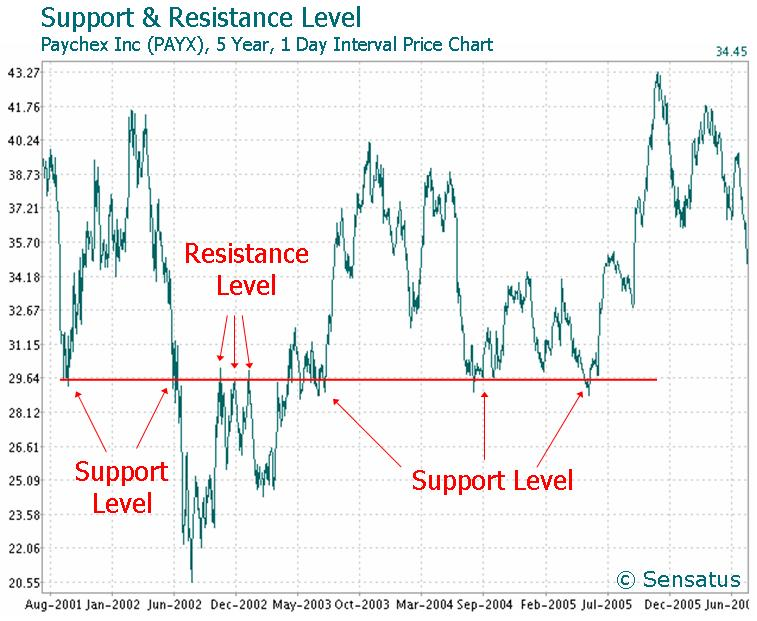
\includegraphics[width=0.8\textwidth]{graphics/fingrundlagen/payx_sup_res.JPG}
	\caption[Paychex Inc. Support Resistance]{Paychex Inc. 5-Jahres-Chart mit 1-Wochen-Intervallen; Level wechselt zwischen Support- und Resistance-Funktion}
	\label{fig:payx_sup_res}
\end{figure}